%%%%%%%%%%%%%%%%%%%%%%%%%%%%%%%%%%%%%%%%%%%%%%%%%%%%%%%%%%%%%%%%%%%%%%
% Trabalho Prático - Grafos 2025/1
% Rede de Água de Belo Horizonte: Modelagem e Cálculo de Fluxo Máximo
% Integrantes: Pedro Porto, Thiago Cury, Vitor Rebula,
%              Lucas Giovine, Guilherme Rodrigues
%%%%%%%%%%%%%%%%%%%%%%%%%%%%%%%%%%%%%%%%%%%%%%%%%%%%%%%%%%%%%%%%%%%%%%

\documentclass[12pt]{article}
\usepackage{float}
\usepackage{sbc-template}
\usepackage{graphicx,url}
\usepackage[utf8]{inputenc}

\sloppy

\title{Cálculo de Fluxo Máximo em Grafos\\
       a partir da Rede de Água de Belo Horizonte}

\author{Pedro Porto, Thiago Cury, Vitor Rebula, Lucas Giovine, Guilherme Rodrigues}

\address{Pontifícia Universidade Católica de Minas Gerais (PUC Minas)\\
         Escola de Engenharia de Computação\\
         Belo Horizonte -- MG -- Brasil\\
         \email{https://github.com/Guilhermeh-R/Grafos}}

\begin{document}

\maketitle

\begin{abstract}
  This work presents a heuristic-based approach to improve water distribution networks by modeling them as directed and weighted graphs. Initially, we attempted to use official CSV data from Belo Horizonte’s open data portal. However, due to performance limitations and the complexity of processing real-world data, we shifted to generating our own CSV manually. This approach also proved inadequate, as it introduced inconsistencies and lacked the structure needed for algorithmic processing. Ultimately, we adopted a synthetically generated graph, which allowed for greater control and clarity over the topology and flow characteristics. The network was defined with vertices and edges representing segments with average capacities. We implemented the Edmonds–Karp algorithm in Python to calculate the maximum flow between selected sources and demands. Based on the results, our heuristic identifies the most restrictive segment (bottleneck) and simulates its improvement to evaluate the impact on overall flow. The methodology proved effective and aligns with the objectives of the Graph Theory course (2025/1).
\end{abstract}

\begin{resumo}
  Este relatório descreve uma abordagem heurística para sugerir melhorias em redes de distribuição de água, modeladas como grafos dirigidos e ponderados. Inicialmente, utilizamos dados CSV oficiais da Prefeitura de Belo Horizonte, mas, devido à complexidade e ao volume dessas informações, que impactaram negativamente o desempenho do sistema, descartamos essa abordagem. Em uma segunda tentativa, elaboramos manualmente um CSV com dados fictícios, mas essa solução também se mostrou inadequada, pois não refletia corretamente a estrutura esperada pela modelagem. Diante disso, optamos por gerar sinteticamente o grafo, definindo vértices e arestas com capacidades médias controladas. Aplicamos o algoritmo de Edmonds–Karp para calcular o fluxo máximo entre fontes e demandas. Com base nesse resultado, nossa heurística identifica o principal gargalo da rede e simula o impacto de sua ampliação na eficiência do sistema.
\end{resumo}

\section{Contextualização e Motivação}

Este trabalho foi desenvolvido no contexto da disciplina de Grafos (2025/1) e tem como objetivo propor uma heurística para identificar melhorias estruturais em redes de distribuição de água. A ideia central é modelar a rede como um grafo dirigido e ponderado, aplicar algoritmos clássicos da Teoria dos Grafos e, a partir dos resultados, sugerir intervenções que maximizem a eficiência da rede. O foco do grupo foi o \textbf{Tema 4 — Monitoramento de distribuição de água}, com ênfase na análise de gargalos operacionais em áreas urbanas de alta densidade populacional.

A motivação partiu da observação do crescimento acelerado da verticalização em Belo Horizonte, onde a construção de edifícios cada vez mais altos pressiona a infraestrutura existente. Redes antigas, muitas vezes projetadas para cenários menos exigentes, podem conter trechos com capacidade reduzida que limitam o escoamento de água, criando pontos críticos no abastecimento.

Inicialmente, utilizamos dados oficiais da Prefeitura de Belo Horizonte (PBH), disponibilizados em formato CSV, os quais descrevem trechos da rede com coordenadas geográficas e larguras das tubulações. Com essas informações, tentamos construir um grafo em que os vértices seriam deduzidos a partir das coordenadas (com aplicação de \textit{snap} para deduplicação), e as arestas receberiam pesos com base nas larguras médias dos segmentos.

Contudo, ao processar essa base, nos deparamos com sérias dificuldades técnicas: a fragmentação e a falta de conectividade dos dados impossibilitaram a execução adequada de algoritmos como Edmonds–Karp, que exigem grafos fortemente conectados. Em um segundo momento, tentamos contornar essas limitações criando um CSV manualmente, com trechos fictícios interligados. No entanto, essa abordagem também se mostrou ineficaz, pois a estrutura dos dados ainda não refletia um grafo utilizável de forma confiável.

Diante disso, optamos por gerar um grafo sintético, totalmente conectado, baseado na lógica estrutural observada em redes reais, mas com controle total sobre a topologia e as capacidades dos trechos. Essa decisão nos permitiu conduzir os testes e validar a heurística em um ambiente simulado, mas condizente com os desafios do problema original.

A partir dessa rede simulada, o projeto evoluiu para uma proposta de heurística baseada na identificação e ampliação do menor gargalo da rede — ou seja, o trecho com a menor capacidade no caminho de maior fluxo. Ao aumentar iterativamente esse gargalo e recalcular o fluxo, buscamos mensurar o impacto direto de uma melhoria pontual e propor, com base em evidências computacionais, qual seria a intervenção mais eficaz na rede.

Dessa forma, o projeto não apenas reforça o entendimento prático dos algoritmos de fluxo máximo, mas também propõe um caminho realista e replicável para otimização de redes urbanas por meio de simulações computacionais.


\section{Referencial Teórico}

\subsection{Fluxo Máximo}

O problema do fluxo máximo é um dos principais tópicos na teoria dos grafos aplicados a redes de transporte, comunicação e logística. Seu objetivo é determinar o maior fluxo possível que pode ser enviado de um vértice origem \( s \) a um vértice destino \( t \) em um grafo direcionado, respeitando as capacidades máximas das arestas. Cada aresta da rede possui uma capacidade que limita o quanto de fluxo pode atravessá-la, e a quantidade de fluxo que entra em um vértice (excetuando \( s \) e \( t \)) deve ser igual à quantidade que sai dele \cite{ahuja1993network}.

Esse problema possui aplicações práticas em diversas áreas, como alocação de recursos, planejamento de produção, logística e otimização de redes urbanas. No presente trabalho, aplicamos o conceito de fluxo máximo para modelar e analisar redes de distribuição de água, visando identificar gargalos e propor melhorias que aumentem a eficiência do sistema.

\subsection{Rede Residual}

A rede residual é um conceito essencial para a resolução de problemas de fluxo máximo. Trata-se de uma representação derivada da rede original, que indica as possibilidades de aumentar ou reduzir o fluxo em cada aresta, com base no fluxo atual. Para cada aresta \( (u, v) \) com capacidade \( c(u, v) \) e fluxo atual \( f(u, v) \), a rede residual inclui:

\begin{itemize}
  \item Uma aresta direta \( (u, v) \) com capacidade residual \( c(u, v) - f(u, v) \), representando quanto ainda pode ser adicionado;
  \item Uma aresta reversa \( (v, u) \) com capacidade \( f(u, v) \), permitindo reverter parte do fluxo já adicionado.
\end{itemize}

Essa estrutura permite identificar caminhos aumentantes – sequências de arestas com capacidade residual positiva – que podem ser utilizados para incrementar o fluxo total. A cada iteração do algoritmo, a rede residual é atualizada, até que não haja mais caminhos aumentantes disponíveis \cite{cormen2009}.

\subsection{Algoritmo de Edmonds-Karp}

O algoritmo de Edmonds-Karp é uma implementação do método de Ford-Fulkerson para resolver o problema do fluxo máximo, que utiliza busca em largura (BFS) para encontrar caminhos aumentantes na rede residual. A vantagem dessa abordagem é que, ao sempre escolher o caminho com o menor número de arestas, ela garante uma complexidade polinomial de \( O(VE^2) \), onde \( V \) representa o número de vértices e \( E \), o número de arestas \cite{edmonds1972}.

A cada iteração, o algoritmo realiza uma busca em largura para encontrar um caminho aumentante do vértice origem ao vértice destino. Em seguida, determina o gargalo do caminho – a menor capacidade residual entre as arestas do caminho – e ajusta o fluxo e a rede residual de acordo. Esse processo se repete até que não existam mais caminhos aumentantes, momento em que o fluxo máximo é atingido.

Por sua eficiência e clareza conceitual, o algoritmo de Edmonds-Karp foi utilizado neste projeto como base para o desenvolvimento de uma solução computacional voltada à otimização de alocação de recursos na instituição parceira.

\nocite{ahuja1993network,cormen2009,edmonds1972}



\section{Modelagem da Solução}

A modelagem da solução foi essencial para estruturar de forma clara e modular as funcionalidades e componentes do projeto. Como o trabalho envolve a leitura de dados de rede, construção de um grafo direcionado e ponderado, execução de um algoritmo de fluxo e simulação de melhorias com base em gargalos, optamos por documentar o sistema com três diagramas principais: \textit{caso de uso}, \textit{atividades} e \textit{classes}. Estes diagramas foram elaborados para representar tanto o fluxo lógico quanto os componentes internos da aplicação, incluindo a nova funcionalidade de sugestão heurística de melhorias na rede.

\subsection{Diagrama de Caso de Uso}

O diagrama de caso de uso representa as interações externas do usuário com o sistema. O ator \textbf{Usuário} realiza ações como fornecer o arquivo CSV (ou optar por uma rede simulada), selecionar os vértices de origem e destino, executar o cálculo de fluxo máximo e acionar a heurística para recomendação de melhorias.

As funcionalidades principais da aplicação incluem o carregamento e interpretação dos dados da rede, a construção do grafo direcionado e ponderado, a execução do algoritmo de Edmonds–Karp e a sugestão de uma intervenção estrutural pontual, baseada na detecção do menor gargalo da rede residual.

\begin{figure}[H]
\centering
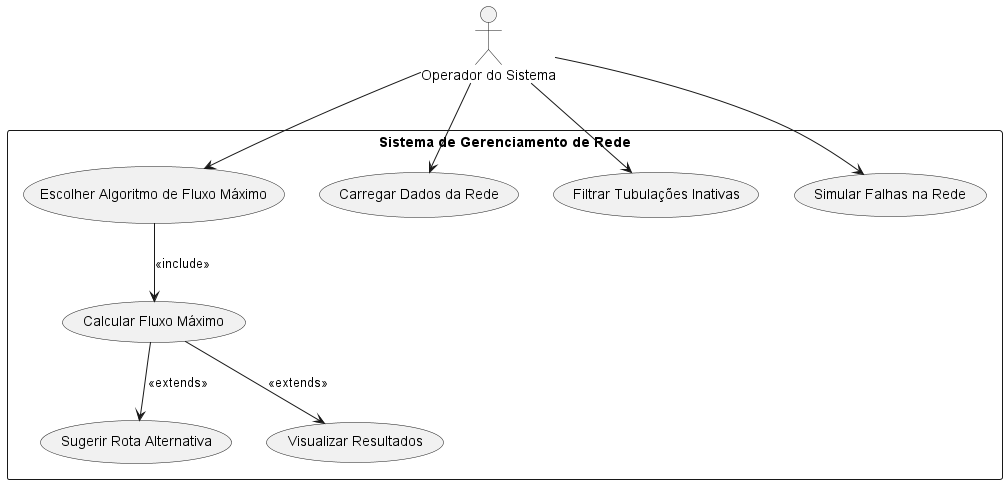
\includegraphics[height=0.7\textheight]{Diagramas/diagrama-caso-de-uso.png}
\caption{Diagrama de Caso de Uso da aplicação.}
\label{fig:caso-uso}
\end{figure}

\subsection{Diagrama de Atividades}

O diagrama de atividades descreve o fluxo operacional da aplicação, desde o fornecimento do arquivo com os dados da rede até a análise da solução final. Após o carregamento do CSV, os dados são filtrados e transformados em vértices e arestas, que compõem o grafo principal.

A seguir, o algoritmo de Edmonds–Karp é executado para encontrar o fluxo máximo entre os vértices definidos pelo usuário. Com base na rede residual gerada, a heurística identifica o gargalo mais limitante — isto é, a aresta com menor capacidade residual que impacta diretamente o fluxo — e simula uma ampliação desse trecho para verificar o ganho potencial na vazão global da rede.

\begin{figure}[H] 
\centering
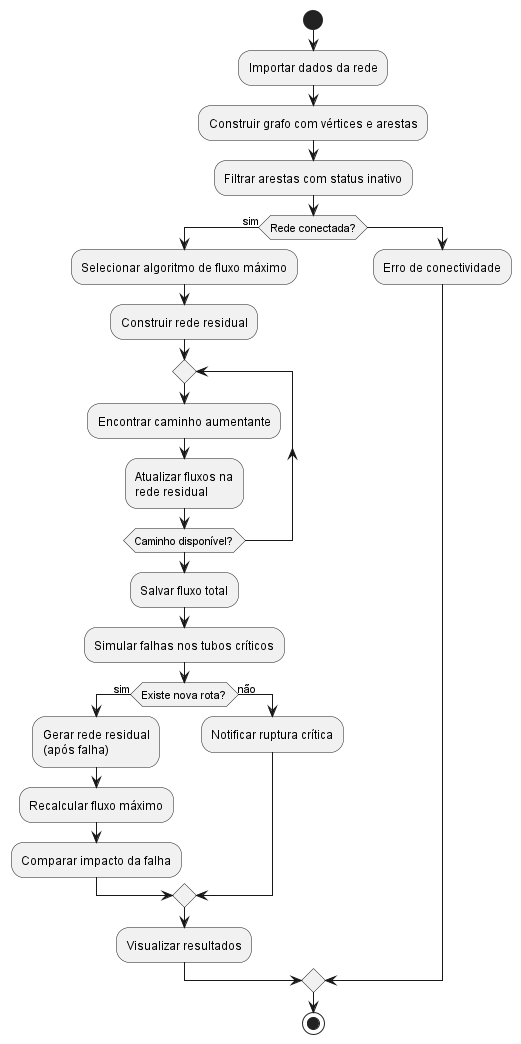
\includegraphics[width=0.8\textwidth]{Diagramas/diagrama-de-atividades.png}
\caption{Fluxo de atividades da aplicação.}
\label{fig:atividades}
\end{figure}

\subsection{Diagrama de Classes}

O diagrama de classes detalha a estrutura interna do sistema e os principais componentes desenvolvidos. Entre as principais entidades, destacam-se:

\begin{itemize}
  \item \texttt{Vertice}: representa os nós do grafo, definidos por coordenadas geográficas X e Y.
  \item \texttt{Trecho}: encapsula as informações de cada linha do CSV, como identificação, coordenadas e largura da tubulação.
  \item \texttt{Grafo}: armazena a estrutura do grafo dirigido, com métodos para adicionar vértices, arestas e calcular fluxo.
  \item \texttt{Algoritmo}: executa o Edmonds–Karp, calcula a rede residual e fornece métodos auxiliares para identificar gargalos.
  \item \texttt{HeuristicaMelhoria}: componente responsável por aplicar a lógica de simulação de melhoria no gargalo e reavaliar o fluxo resultante.
\end{itemize}

A modularização favoreceu a manutenção do código, a implementação de testes e a extensão das funcionalidades ao longo do desenvolvimento.

\begin{figure}[H]
\centering
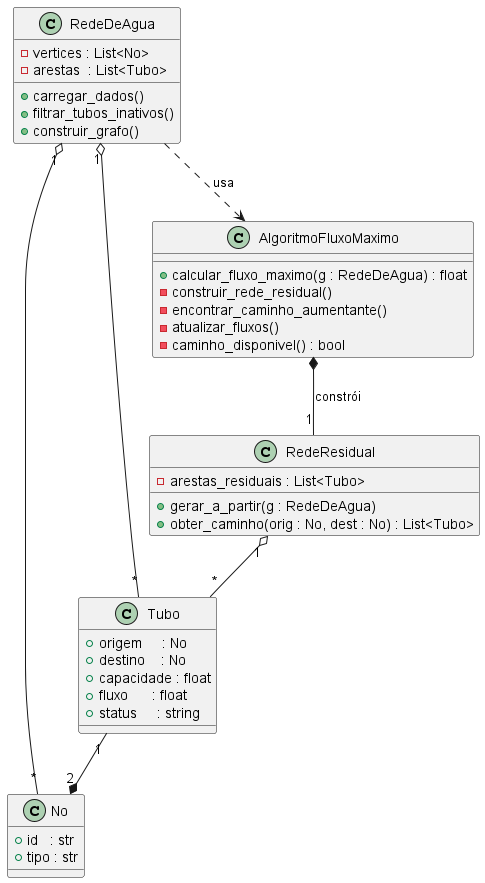
\includegraphics[height=0.6\textheight]{Diagramas/diagrama-classes.png}
\caption{Diagrama de Classes utilizado na implementação.}
\label{fig:classes}
\end{figure}

\section{Desafios e Ajustes Metodológicos}

Durante o desenvolvimento do projeto, nos deparamos com desafios práticos relacionados à qualidade e conectividade dos dados reais da rede de água de Belo Horizonte, disponibilizados pela PBH. Inicialmente, a intenção era utilizar exclusivamente essa base para representar o sistema real de distribuição e aplicar os testes de fluxo máximo. No entanto, após a leitura e interpretação dos dados, identificamos que muitos trechos não estavam devidamente conectados entre si, comprometendo a formação de um grafo coeso.

Esse problema inviabilizou a aplicação direta da nossa metodologia, que pressupõe uma estrutura conectada para que o algoritmo de Edmonds–Karp funcione corretamente. Diante disso, optamos por construir uma base simulada, com uma rede fictícia porém coerente com a lógica de uma rede de escoamento real. A rede simulada foi projetada com conexões funcionais entre os vértices, o que nos permitiu executar os testes com sucesso.

A partir dessa rede funcional, aplicamos o algoritmo de fluxo máximo com o objetivo de identificar o principal gargalo da rede — ou seja, o trecho com menor capacidade que mais limita o escoamento total. Após identificar esse gargalo, realizamos uma simulação para medir o impacto da melhoria pontual apenas nesse trecho específico, como se sua capacidade fosse ampliada. Essa abordagem permite avaliar de forma objetiva como uma única intervenção pode influenciar a eficiência do sistema como um todo.

Apesar da limitação enfrentada com os dados reais, a abordagem adotada permitiu validar a lógica do algoritmo e demonstrar, mesmo que em um cenário hipotético, como simulações computacionais podem apoiar decisões sobre manutenção e expansão de redes urbanas. Os resultados finais apresentados neste relatório foram obtidos a partir da base sintética com 100 vértices, gerada artificialmente para esse fim.

\subsection{Primeiros Testes com a Base Oficial da PBH}

Na fase inicial da pesquisa, buscamos compreender a estrutura dos dados fornecidos pela Prefeitura de Belo Horizonte (PBH), disponíveis em formato CSV. Para isso, carregamos um subconjunto com apenas 10 linhas do arquivo original, o que nos permitiu realizar os primeiros testes de geração do grafo e validação da conectividade.

A Figura~\ref{fig:grafo_pbh} mostra o grafo gerado a partir dessas 10 linhas. Nele, os vértices foram criados a partir das coordenadas extraídas do campo \texttt{GEOMETRIA}, presente em cada trecho. Cada coordenada foi convertida em um identificador único por meio de um \textit{snap} com arredondamento, garantindo que pontos coincidentes fossem reconhecidos como o mesmo vértice.

\begin{figure}[H]
\centering
\includegraphics[width=0.85\textwidth]{grafos/PBH-10_trechos.jpg}
\caption{Grafo gerado com 10 trechos do CSV da PBH.}
\label{fig:grafo_pbh}
\end{figure}

Observa-se que grande parte dos trechos se comporta de forma isolada, formando pequenos grupos de vértices não conectados. Esse comportamento evidencia um problema de conectividade na base real: mesmo em uma pequena amostra, os dados não formam um grafo coeso, o que inviabiliza análises globais de fluxo.

Além da construção dos vértices, também definimos as arestas com base nas coordenadas de cada trecho. O peso de cada aresta foi determinado pela média entre os campos \texttt{LARG\_INICIO} e \texttt{LARG\_FINAL}, ambos disponíveis na tabela original. Esse valor foi interpretado como a capacidade de transporte de água do respectivo trecho.

Essas definições de modelagem — extração de vértices a partir do campo de geometria e uso da largura como peso das arestas — foram mantidas mesmo nos testes com a rede simulada, garantindo consistência na metodologia adotada ao longo do projeto.

\subsection{Simulação na Interface Gráfica e Heurística Adotada}

Diante da complexidade e do volume elevado da base oficial fornecida pela Prefeitura de Belo Horizonte — que conta com mais de 50 mil registros —, identificamos limitações técnicas para a execução eficiente das simulações dentro do sistema desenvolvido. O carregamento e o processamento integral desses dados demandariam otimizações adicionais e infraestrutura computacional mais robusta, o que inviabilizaria a realização prática dos testes no escopo deste projeto. Assim, optou-se pela construção de uma base de dados própria e controlada, com volume reduzido e estrutura simplificada, mas ainda representativa em termos de conectividade e capacidades. Essa abordagem permitiu validar os algoritmos implementados, ajustar a modelagem do grafo e assegurar a estabilidade da interface gráfica, mantendo a fidelidade à lógica do problema original.

Com isso, a partir da base simulada e dos testes realizados, foi possível desenvolver uma interface gráfica para facilitar a visualização e simulação dos diferentes fluxos possíveis dentro da rede. A Figura~\ref{fig:menu_acoes} mostra a tela inicial da aplicação, onde o usuário seleciona os vértices de origem e destino, além de escolher as opções desejadas.

\begin{figure}[H]
\centering
\includegraphics[width=0.6\textwidth]{grafos/Menu grafos.png}
\caption{Menu da aplicação com as opções disponíveis para o usuário, como adicionar vértices, arestas e executar o algoritmo de fluxo máximo.}
\label{fig:menu_acoes}
\end{figure}

A Figura~\ref{fig:grafo_exibido} ilustra a interface gráfica da aplicação com um grafo montado pelo usuário. Cada vértice pode ser arrastado livremente e as arestas são exibidas com as respectivas capacidades, permitindo uma compreensão visual da estrutura da rede.

\begin{figure}[H]
\centering
\includegraphics[width=0.6\textwidth]{grafos/Exibir grafo.png}
\caption{Visualização gráfica do grafo construído pelo usuário, com vértices e arestas posicionados interativamente na tela.}
\label{fig:grafo_exibido}
\end{figure}

A Figura~\ref{fig:fluxo_maximo} mostra a visualização do grafo com o fluxo máximo calculado para o caminho selecionado. Os fluxos estão indicados nas arestas com a notação \texttt{fluxo/capacidade}.

\begin{figure}[H]
\centering
\includegraphics[width=0.95\textwidth]{grafos/Fluxo Máximo.png}
\caption{Resultado da simulação de fluxo máximo.}
\label{fig:fluxo_maximo}
\end{figure}

Com base no resultado do fluxo, adotamos como heurística a identificação do menor gargalo (trecho com menor capacidade residual crítica) e a simulação da ampliação pontual dessa aresta. A Figura~\ref{fig:sugestao_melhoria} apresenta o resultado da análise, destacando em azul a aresta cuja ampliação teria o maior impacto positivo no fluxo total da rede.

\begin{figure}[H]
\centering
\includegraphics[width=0.95\textwidth]{grafos/Menor Gargalo.png}
\caption{Sugestão de melhoria: ampliação da capacidade no menor gargalo.}
\label{fig:sugestao_melhoria}
\end{figure}

Essa abordagem permite fornecer ao usuário uma recomendação objetiva e automatizada sobre onde intervir na rede para obter maior eficiência, contribuindo com decisões de manutenção ou expansão mais assertivas.

\subsection{Simulação em Grafo Sintético}

Para validar a robustez da solução desenvolvida, foram realizados testes em um grafo sintético contendo 50 vértices, com conectividade e capacidades atribuídas aleatoriamente, mas respeitando a lógica de uma rede de escoamento realista. A Figura~\ref{fig:grafo_sintetico_50} apresenta esse grafo com todas as conexões e capacidades visíveis, permitindo a inspeção da estrutura e dos caminhos possíveis.

\begin{figure}[H]
\centering
\includegraphics[width=0.95\textwidth]{grafos/grafo sintetico 50 vertices.jpeg}
\caption{Grafo sintético com 50 vértices, utilizado para simulações de fluxo máximo.}
\label{fig:grafo_sintetico_50}
\end{figure}

A Figura~\ref{fig:fluxo_maximo_sintetico} mostra o resultado da simulação do fluxo máximo no grafo sintético, evidenciando em vermelho o caminho percorrido com a vazão máxima obtida entre os nós de origem e destino definidos. As arestas exibem os valores de fluxo efetivo em relação à capacidade total (\texttt{fluxo/capacidade}), reforçando a compreensão visual dos gargalos da rede.

\begin{figure}[H]
\centering
\includegraphics[width=0.95\textwidth]{grafos/fluxo maximo sintetico.jpeg}
\caption{Fluxo máximo calculado no grafo sintético com 50 vértices.}
\label{fig:fluxo_maximo_sintetico}
\end{figure}



\section{Resultados}

Na presente análise, foram selecionadas duas coordenadas específicas correspondentes a vértices da rede, com o objetivo de avaliar o comportamento do fluxo de água entre esses pontos. A partir dessas coordenadas, construiu-se a rede residual associada, possibilitando o cálculo do fluxo máximo viável na rede, considerando suas capacidades atuais. Esse procedimento permitiu a identificação precisa do gargalo — o trecho de menor capacidade que limita o escoamento total entre os vértices analisados. Tal identificação é fundamental para direcionar intervenções estruturais estratégicas visando a melhoria da eficiência da infraestrutura.

Com base nesses resultados, foi proposta a implementação de uma interface gráfica interativa, capaz de simular a ampliação da capacidade especificamente no menor gargalo identificado. Essa visualização facilita tanto a compreensão técnica do problema quanto a tomada de decisão por parte de gestores públicos ou engenheiros responsáveis. Dessa forma, a metodologia aplicada não apenas confirma a eficácia do algoritmo utilizado para o cálculo do fluxo máximo e a detecção de pontos críticos, como também oferece um recurso prático para o planejamento e otimização de redes hidráulicas urbanas.

\section{Conclusão}

Este trabalho teve como objetivo aplicar conceitos da Teoria dos Grafos para modelar, analisar e propor melhorias em redes de distribuição de água, utilizando como referência inicial os dados reais da rede de Belo Horizonte. No entanto, devido a limitações de conectividade presentes na base oficial, optou-se pela construção de uma rede simulada, inspirada em sistemas reais, mas com estrutura controlada e conectividade garantida, o que permitiu a aplicação prática dos algoritmos estudados.

A modelagem da rede como um grafo direcionado e ponderado possibilitou a aplicação do algoritmo de Edmonds–Karp para o cálculo do fluxo máximo entre dois pontos definidos pelo usuário. A principal contribuição do projeto, entretanto, reside na heurística desenvolvida: a identificação do menor gargalo (isto é, a aresta de menor capacidade crítica na rede residual) e a simulação da ampliação desse trecho para mensurar o impacto direto no desempenho global da rede.

Os resultados demonstram que, mesmo em uma rede simulada, é possível identificar pontos de estrangulamento e propor intervenções localizadas que resultam em ganhos expressivos de eficiência. Essa abordagem evidencia como algoritmos clássicos da teoria dos grafos, aliados a visualizações interativas, podem apoiar decisões de planejamento, manutenção e expansão de infraestruturas urbanas.

Além de reforçar o aprendizado prático de algoritmos de fluxo máximo, o projeto destaca o potencial da modelagem computacional e de simulações heurísticas como ferramentas para o diagnóstico e a otimização de sistemas complexos. Trabalhos futuros poderão explorar melhorias na heurística utilizada, considerar restrições orçamentárias nas intervenções ou adaptar a metodologia para outros tipos de redes, como as de transporte, energia ou saneamento.



\bibliographystyle{sbc}
\bibliography{refs}

\end{document}